\section{Experimental Setup}

\begin{frame}{Overview} % ______________________________________________________
  \hspace*{-12.5mm}
  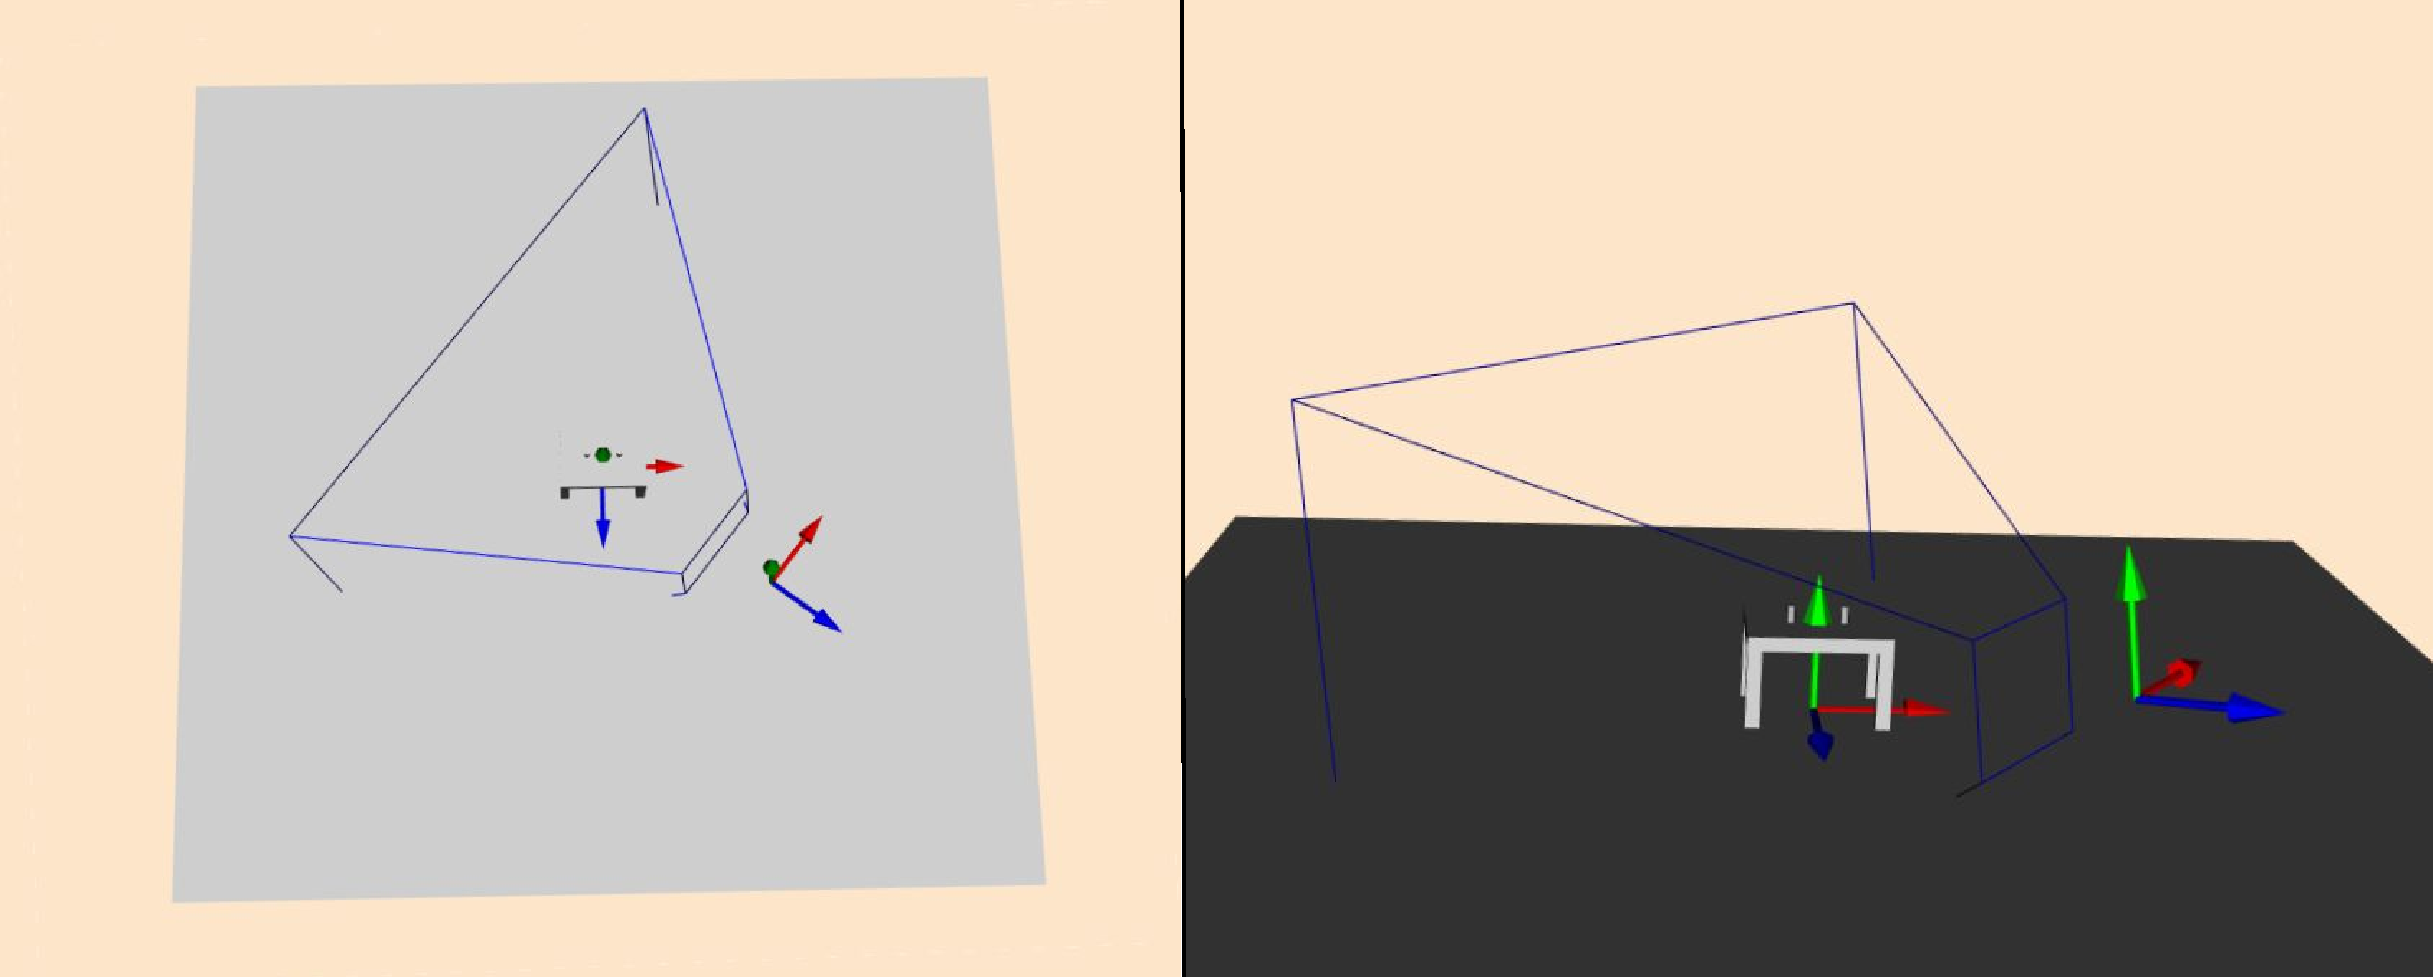
\includegraphics[width=1.2\textwidth]
    {../figures/expsetup_simulation_overview.pdf}
  \note{\begin{itemize}
    \item ** All experiments done in a simulation environment
    \item Third person view of simulation environment
    \item[] Two main coordinate systems
    \item A coordinate system fixed to the environment called the global
    coordinate system
    \item One attached the origin of the sensor's viewing frustum
    \item[] red, green, and blue arrows represent the x, y, and z axis
    respectively
  \end{itemize}}
\end{frame}

\subsection{Simulated Sensor}

\begin{frame}{Simulating a RGB-D Sensor} % _____________________________________
  \begin{itemize}
    \item Adding noise to the depth image
    \item Sensor path
  \end{itemize}

  \note{\begin{itemize}
    \item First I will discuss
    \item Adding noise to the depth image to simulate a depth sensor in a real environment
    \item Second I will discuss
    \item The path the sensor takes in each experiment
  \end{itemize}}
\end{frame}

\begin{frame}{Rendering Pipeline} % ____________________________________________
  \hspace*{-12.5mm}
  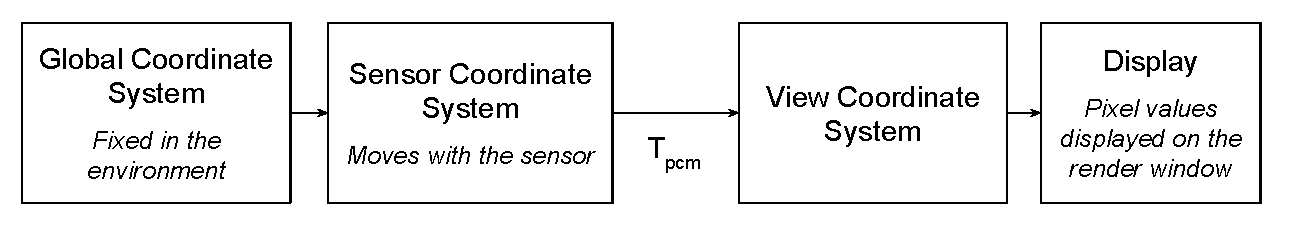
\includegraphics[width=1.2\textwidth]
    {../figures/expsetup_render_pipeline.pdf}
  \note{\begin{itemize}
    \item Pinhole camera model
    \item transforms geometry in the sensor's coordinate system to homogenous
    coordinates
    \item z-component of the homogenous coordinates is what defines the depth
    image
  \end{itemize}}
\end{frame}

\begin{frame}{$T_{pcm}$} % _____________________________________________________
  \vspace{-0.15in}
  \begin{center}
  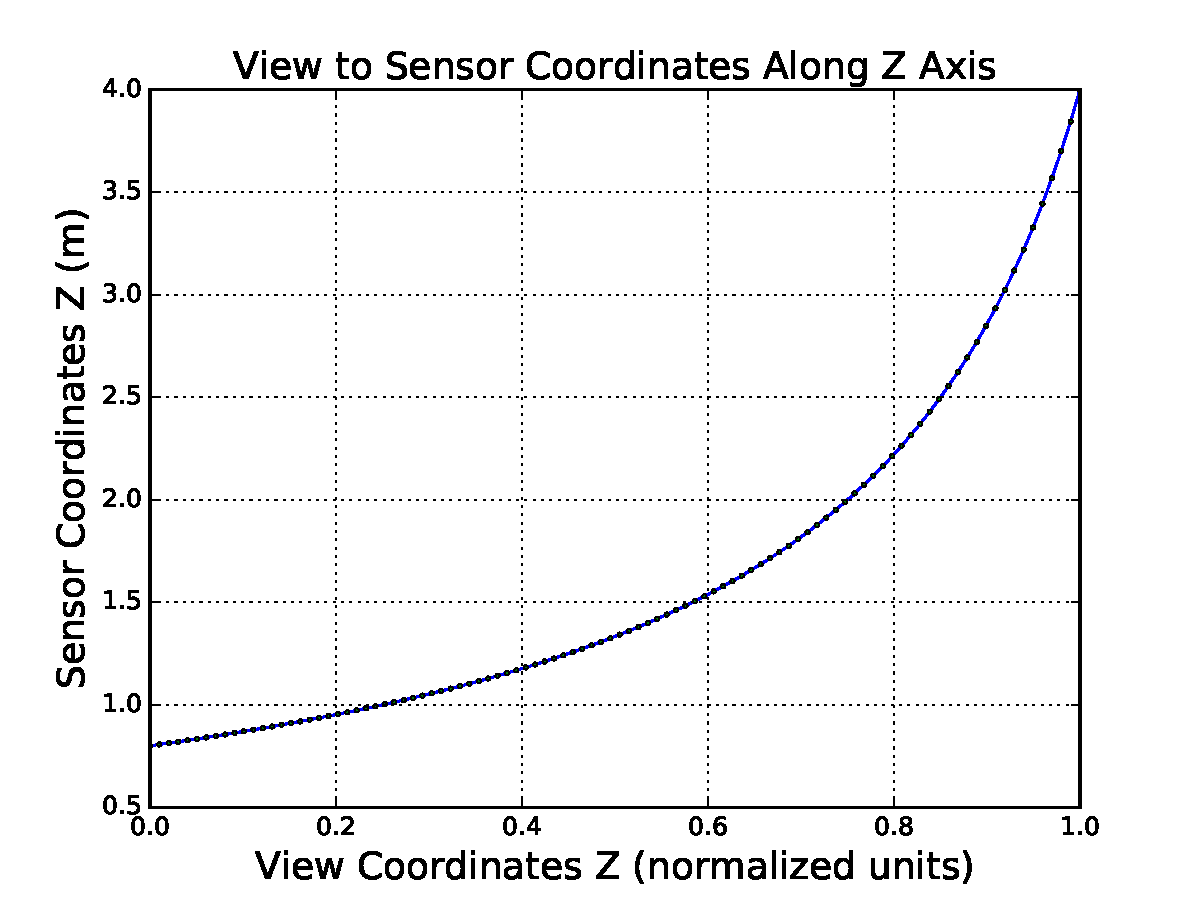
\includegraphics[height=0.90\textheight]
    {../figures/expsetup_depth_view_to_sensor.pdf}
  \end{center}
  \note{\begin{itemize}
    \item The pinhole camera transformation, $T_{pcm}$,
    \item Creates a non-linear relationship between
    \item - values in the depth image
    \item - and their corresponding location in the sensor's coordinate system
    \item Graph was created by:
    \item - Taking center pixel in depth image
    \item - Varying value 0-1 and projecting to camera's coordinate system
  \end{itemize}}
\end{frame}

\begin{frame}{Adding Noise} % __________________________________________________
  \only<1>{\vspace{-0.15in}\begin{center}
  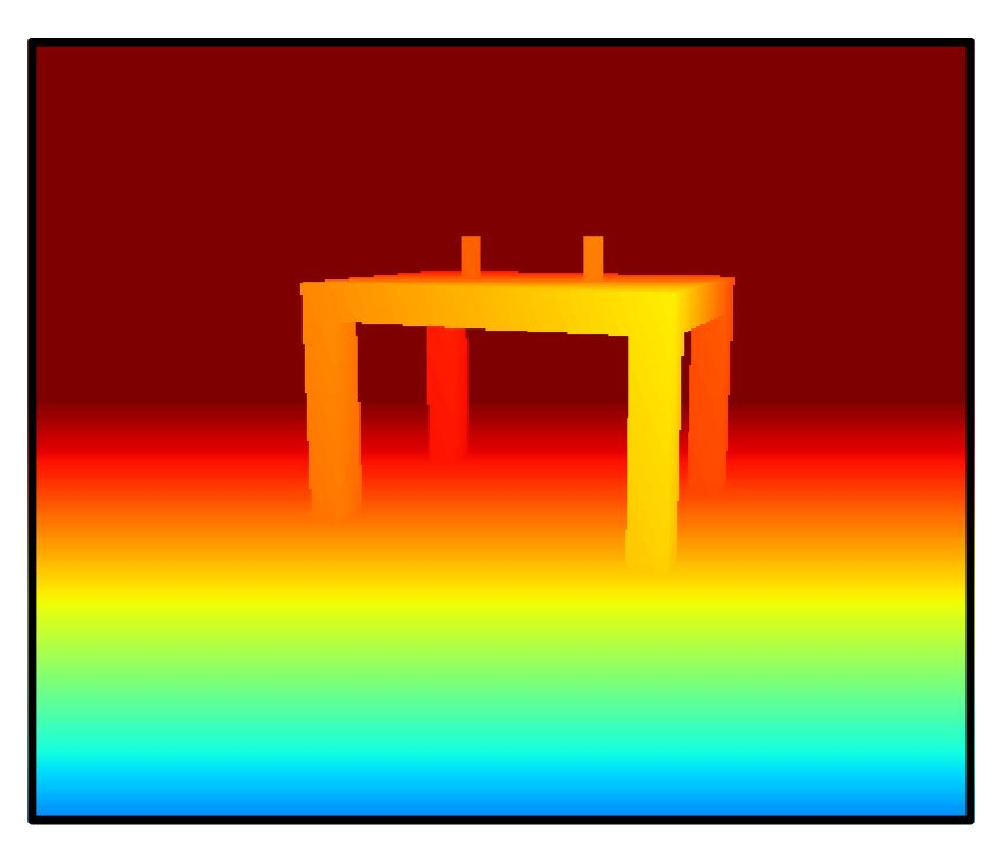
\includegraphics[height=0.90\textheight]
    {../figures/presentation/approach_depth_image_p.pdf}
  \end{center}}

  \only<2>{\begin{center}
    $D_{noisy}(i,j) = D(i,j) + \mathcal{N} (\mu\mathsmaller{=}0, \sigma\mathsmaller{=}0.002)$
  \end{center}}

  \only<3>{
  K. Khoshelham and S. O. Elberink, "Accuracy and resolution of Kinect depth
  data for indoor mapping applications." \emph{Sensors (Basel, Switzerland)}
  \medskip
  \begin{center} $\sigma_z = 1.425\mathrm{e}{-5} \times Z^2$ \end{center}
  }

  \only<4>{\vspace{-0.15in}\begin{center}
  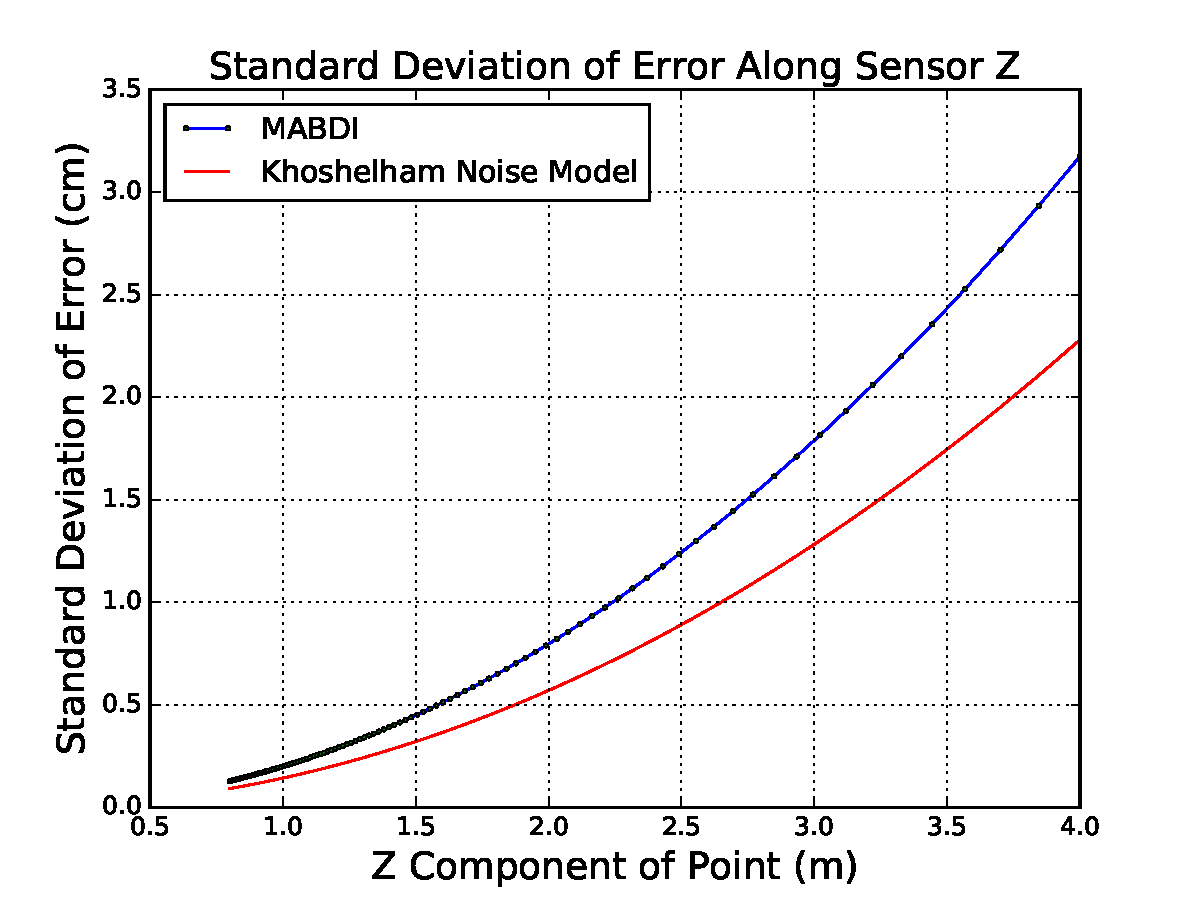
\includegraphics[height=0.90\textheight]
    {../figures/expsetup_noise_error.pdf}
  \end{center}}

  \note<1>{\begin{itemize}
    \item The depth image
    \item[]
    \item I am going to describe how to take a "noiseless" depth image
    \item and add noise to mimic a real RGB-D sensor in the real world
  \end{itemize}}
  \note<2>{\begin{itemize}
    \item I sample a normal distribution and add the value to each pixel
  \end{itemize}}
  \note<3>{\begin{itemize}
    \item Researchers have created error models to describe the standard
    deviation of measurement error found in various RGB-D sensors
    \item Point in camera's coordinate system
    \item Point has some z value $Z$
    \item $\sigma_z$ - standard deviation of error
    \item as a function of $Z$
  \end{itemize}}
  \note<4>{\begin{itemize}
    \item Each line shows how the measurement's standard deviation of error
    changes as the point moves along the z axis in the sensor's coordinate
    system.
    \item The standard deviation of error simulated in our experiments is larger
    than that defined by Khoshelham's model for points within the sensor's
    range.
  \end{itemize}}
\end{frame}

\begin{frame}{Sensor Path} % __________________________________________________
  \vspace{-0.25in}
  \begin{center}
  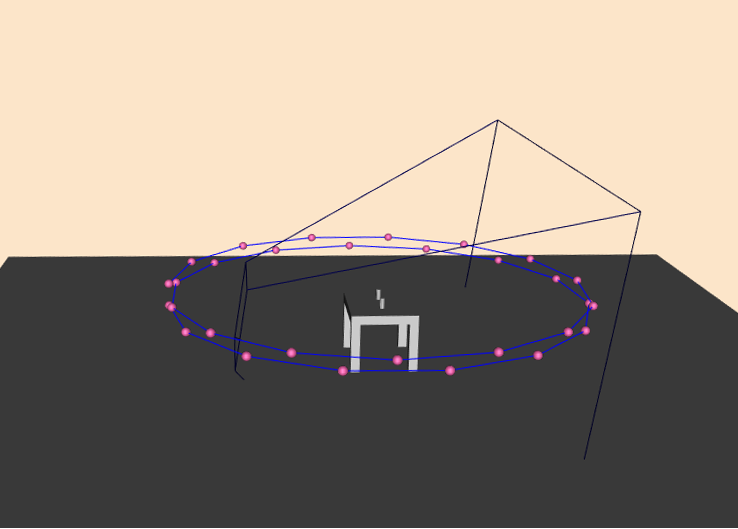
\includegraphics[height=0.90\textheight]
    {../figures/expsetup_path.png}
  \end{center}
\end{frame}

\note[itemize]{
\item blue line indicates the path
\item pink points indicate where the sensor stops along the path
\item path circles the objects in the environment twice
\item[] Helical path was chosen
\item - it returns to a part of the environment that has already been mapped and
is thus ``known'' to the algorithm
\item - helix so views the environment from a slightly different position on
each pass
}

\subsection{Simulation Parameters}

\begin{frame}{Simulation Parameters} % _________________________________________
  \begin{table}[h]
    \begin{center}
      \begin{tabular}{|l|c|c|c|c|}
      \hline
             & Environment & Noise   & Dynamic & Iterations \\\hline
      Experiment 1	 & Table       & False   & False   & 30 \\
      Experiment 2  & Bunnies     & True    & False   & 50 \\
      Experiment 3  & Bunnies     & True    & True    & 50 \\
      \hline
      \end{tabular}
    \end{center}
  \end{table}
  \note{\begin{itemize}
    \item Parameters that control the simulated environment
    \item with chosen values for each run
    \item[] Environment
    \item \textit{Table}
    \item - consists of a table and two cups placed on the table. The table is 1
    meter tall.
    \item - \textit{Bunnies}
    \item - three bunnies around 1.5 meters tall. Created with Stanford Bunny a well
    known data set in computer graphics.
    \item[] Noise - adds noise to the depth image of the simulated sensor
    \item[] Dynamic - adds an object during the simulation
    \item In this experiment a third bunny is added half-way through the simulation
    \item[] Iterations - The number of times MABDI will run. This number is equal to
    the number of stops the sensor makes along the path
    \item Going through like we did in the Algorithms section is also one iteration
  \end{itemize}}
\end{frame}
